\section{Analysis Overview}
\label{sec:analysis_overview}
The first step to performing a precision measurement of the Higgs boson mass (\mH) is to ``observe'' many Higgs bosons.
However, production of a Higgs boson is essentially nonexistent in everyday conditions and is still extremely rare even in the high-energy \pp collisions of the LHC (Chapter~\ref{ch:lhc}).
At a center-of-mass energy of 13\TeV, the total inclusive inelastic cross section of two protons colliding is 70\mb.
% TODO: CITE.
Comparing this to the production cross section of a Higgs boson $\left( \sigma_{\pp \to \PH} = 59\pb \right)$
% (TODO:cite sigma(pptoH) = 59 pb)
shows that a Higgs boson is produced in approximately one out of every \emph{billion} \pp collisions---a rare event indeed.
% TODO CITE

To complicate matters further, the Higgs boson has a \emph{very} short mean lifetime of only $1.6 \tentotheminus{22}\snd$~\cite{particle_data_group_review_2020}.
Thus, the Higgs boson is not directly detected by CMS (Chapter~\ref{ch:cms}) but is instead \emph{inferred} from its stable decay products that enter the various subdetectors.
Among all the fundamental particles so far discovered, the Higgs boson bears the second heaviest mass (approximately 125\GeV), the first belonging to the top quark.
% TODO:possibly refer back to a section where I mention the quarks individually? (Sec.~\ref{sec:sm}).
This gives the scalar boson sufficient energy to decay into at least 9 different final states, where each decay occurs with a different probability---the \emph{branching fraction} or \emph{branching ratio} (\br)---whose value depends on \mH, as shown in Fig.~\ref{fig:higgs_br}.
% \textcolor{red}{MENTION THAT NOT ALL DECAYS MAKE ON-SHELL PARTICLES?}
The question then becomes, \emph{``Which Higgs boson decay mode is most useful for the measurement of \mH?''}.
\begin{figure}[!htbp]
    \begin{center}
        % Figures come from:
        % https://twiki.cern.ch/twiki/bin/view/LHCPhysics/LHCHWG?redirectedfrom=LHCPhysics.LHCHXSWG#Higgs_cross_sections_and_decay_b
		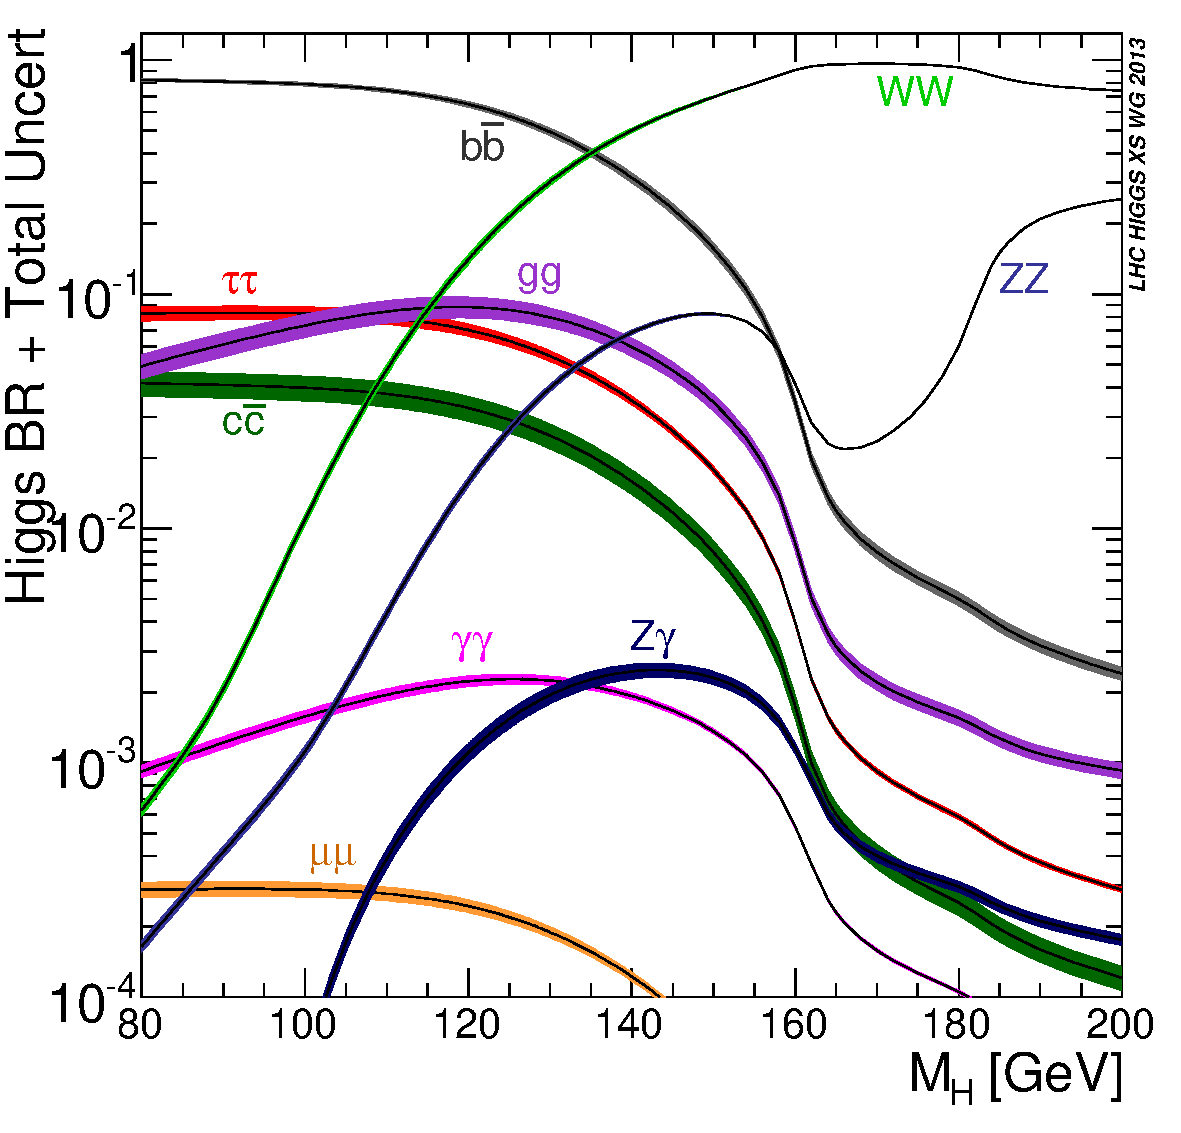
\includegraphics[width=0.48\textwidth]{figures/higgsmassmeas/higgs_BR_80to200GeV.pdf}
		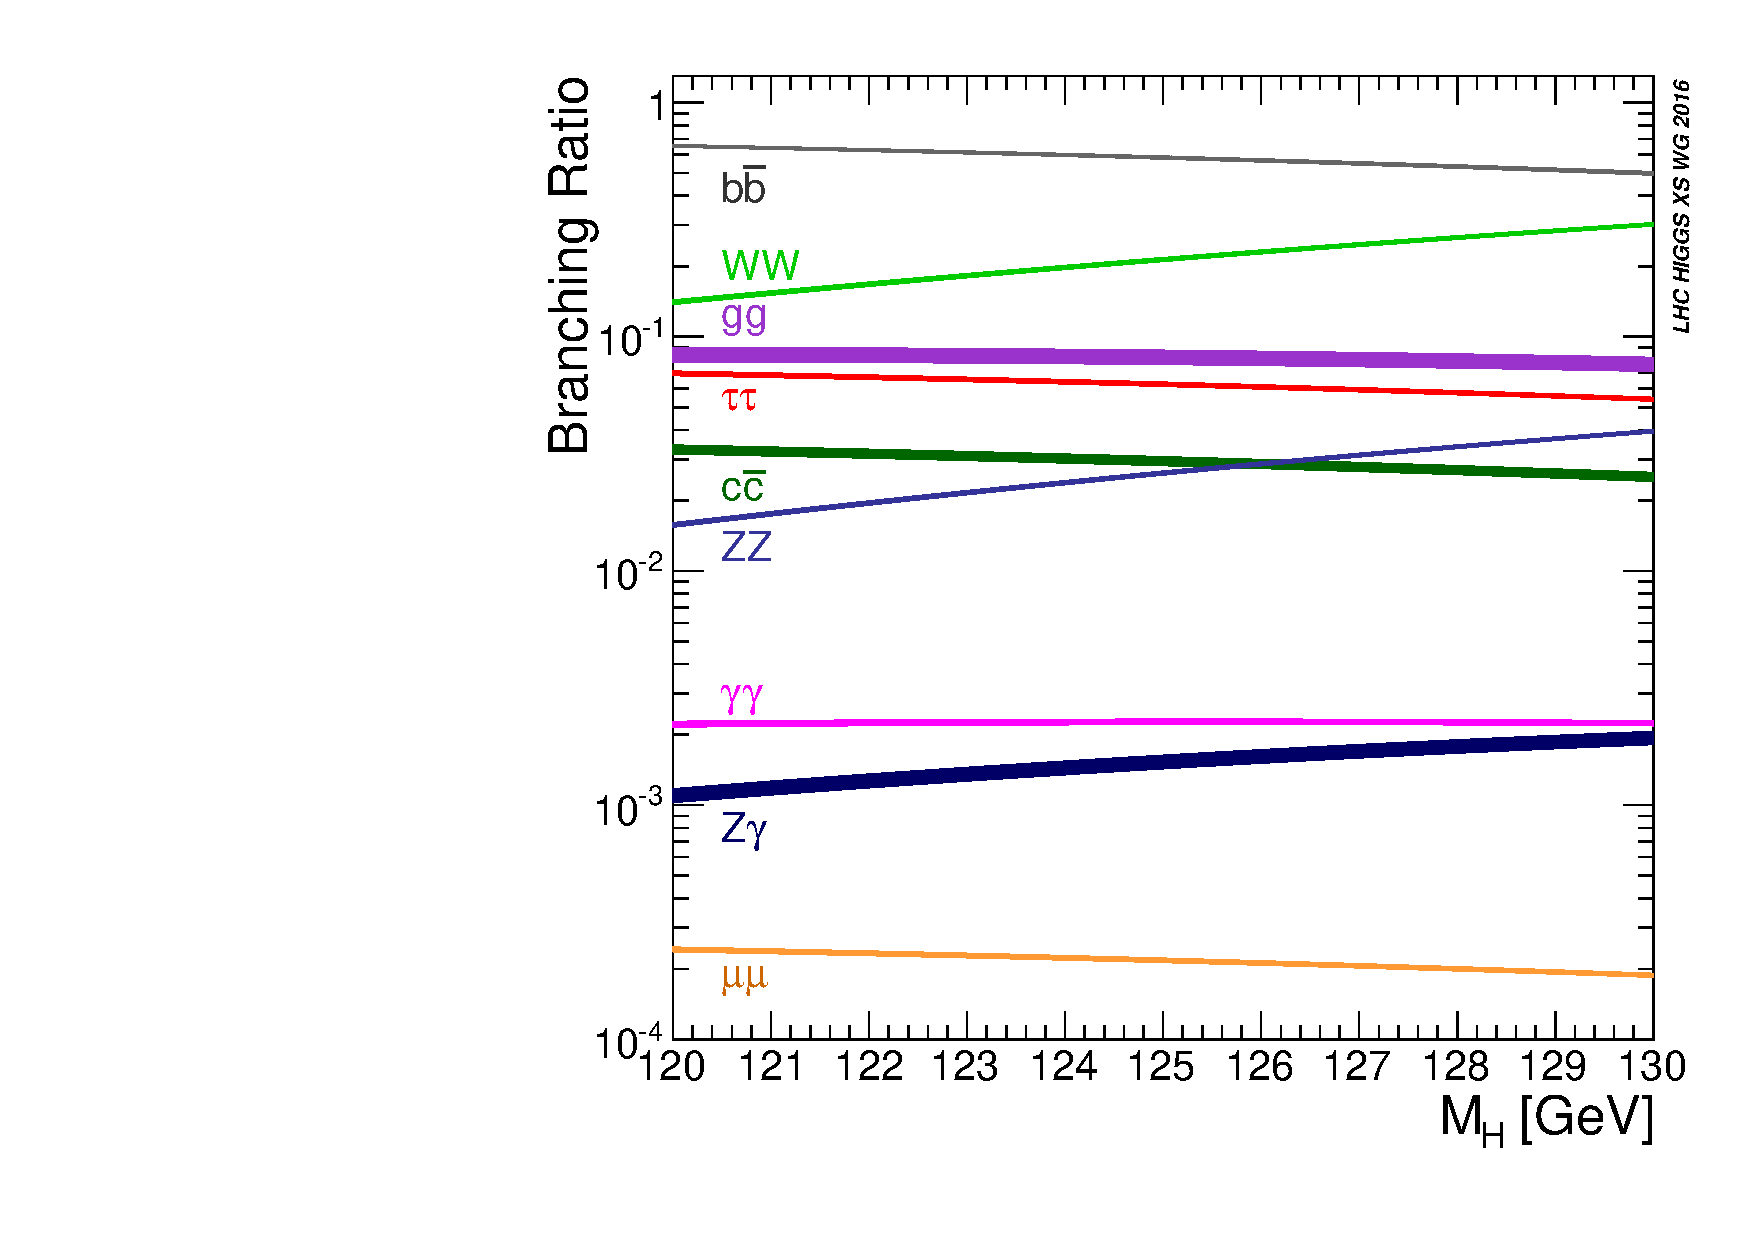
\includegraphics[width=0.48\textwidth]{figures/higgsmassmeas/higgs_BR_120to130GeV.pdf}
		\caption
			[Branching ratios of Higgs boson decays as a function of the Higgs boson mass.]
			{
            The branching ratios of various Higgs boson decays as a function of the Higgs boson mass
            over a wide range (Left) and a narrow range (Right) of values.
            }
		\label{fig:higgs_br}
	\end{center}
\end{figure} 
% Real particles enter detectors in CMS which send signals to various electronics.
% Particle Flow algorithm pieces the information together to construct objects out of each event.
% Now, instead of just a deposit of energy in the ECAL and corresponding hits in the silicon tracker, the particle is identified as a newly produced electron.
% CMS records which kinds of objects came from which events and stores the information in \emph{data sets} (TODO: ref Sec. future).

Owing to its large signal-to-background ratio of approximately 2 and its relatively rare four-lepton final state, the \hzzfourl decay channel is chosen and is called the \emph{signal process}.
On average, a Higgs boson will decay into two \PZ bosons (one on-shell and one off-shell) only 2.6\% of the time.
In turn, each \PZ boson \emph{may} decay into two opposite-sign, same flavor (OSSF) leptons (\Ztolplm, where $\ell = \Pe, \mu$) on average approximately 6.7\% of the time.
This signal process then gives rise to four distinct final states: \foure, \fourmu, \twoetwomu, \twomutwoe.
The branching ratio for the overall signal process is then calculated as: % B(Z->ee)=0.033632, B(Z->mumu)=0.033662
\begin{equation*}
    \BRof{\hzzfourl} = \BRof{\htozz} \left[ \BRof{\Ztolplm} \right]^2 = 1.8\tentotheminus{3}.
\end{equation*}
Thus, a signal event is expected to be produced only once in about every \emph{trillion} \pp collisions.

The strategy is then to search the \pp collision data collected and analyzed by the CMS Experiment for all the detected \hzzfourl events.
The task is not so straightforward;
events in the data are categorized---not by the entire decay process---but by their final state, based on which triggers fired to collect which events.
% TODO: uncomment the line below.
% Section~\ref{sec:datasets_simul_trig} describes the triggers used for this analysis to select events with the \fourl final state found in the corresponding data sets.
For each chosen event, the subdetectors of CMS (Secs.~\ref{sec:tracker}--\ref{sec:solenoid}) provide a plethora of track and energy-detection information to reconstruct \emph{objects}---representations of the underlying particles within the event.
The reconstructed objects are then assembled in a fashion that checks if the logic coincides with the signal process of interest: \hzzfourl.  % TODO: Clean up this sentence.
For example, a pair of OSSF lepton-like objects should appear to come from a \PZ-like object---\ie having a nominal mass of approximately 91\GeV and zero net electric charge---instead of, say, appearing to come from a \PH-like object.
Two such \PZ-like objects must be formed and should appear to come from a \PH-like object.
% OSSF-dilepton objects should each appear to come from a \PZ-boson-like object (\eg having a nominal mass of approximately 91\GeV and zero net electric charge)---instead of, say, coming from a Higgs-boson-like object.
All throughout, the reconstructed event must obey physics conservation laws (energy, momentum, charge, \etc) and the associated objects may even be required to pass certain detector selection criteria (\eg $\pt^\mu > 5\GeV$).
% This process hinges on the conservation of momentum, since in the longitudinal ($z$) direction the \pp collision has initial and final.
% Specifically, the 
%     - The \PZ boson has a precisely measured mass of TODO a neutral particle, so the two leptons into which it decays should combine to Group two leptons together, 
%     - Form two different pairs of opposite-sign, same-flavor (OSSF) leptons
%     - If it appears that the to select specific hzz4l events (\emph{event selection}).
These criteria are analysis-specific and are collectively called the \emph{event selection} of the analysis.
The event selection for this analysis is described in Sec.~\ref{sec:evt_sel}.  % TODO: ref may be wrong.

Although the event selection is constructed to select only signal events, it is not guaranteed;
there are certain physics process that have exactly the same initial and final states as the signal process.
Such processes ``contaminate'' the collected signal events and are called \emph{background processes}.
Concretely, Fig.~\ref{fig:feyndiag_sig_vs_bkg} shows how identical initial state gluons can react to produce exactly the same final state particles, while producing different intermediate particles:
the signal process (Left), initiated by gluon-gluon fusion \vs a background process (Right) which skips the intermediate Higgs boson.
It is imperative for all physics analyses to maximize the number of collected signal events while minimizing the number of collected background events.
Section~\ref{sec:bkg_estim} discusses the associated background processes and how to estimate the number of events these contribute to the signal region.
\begin{figure}[!htbp]
	\begin{center}
		
\includegraphics[width=0.48\textwidth]{figures/placeholder.png}  % TODO.
		
\includegraphics[width=0.48\textwidth]{figures/placeholder.png}  % TODO.
		\caption
			[Feynman diagrams for the \gghzzfourl and \ggzzstarfourl processes.]
			{
            Feynman diagrams showing how the initial and final states are the same
            for the signal process (\gghzzfourl, Left) and one possible background process (\ggzzstarfourl, Right).
			}
		\label{fig:feyndiag_sig_vs_bkg}
	\end{center}
\end{figure}

Before drawing conclusions from the data themselves, it is necessary for particle physicists to make predictions about their analysis using simulated events or \emph{simulation}.
These events simulate a specific process (\eg $\pp \to \hzzfourl$), governed by some theoretical framework that is programmed mathematically into a software package.
% events from simulated particle physics collisions--- are created by software physicists have created software packages that simulate particle physics collisions,
% the resulting particle transformations using various theoretical frameworks,
% and even the interactions that particles have with the virtual detectors, through which they traverse.
Programs like \MGvATNLO and \POWHEG can simulate millions of rare (or even \emph{fictitious}) events in just a single day, whereas the same event in actual data might otherwise take decades---\emph{or not at all!}% might otherwise take many years to observe in data.
Furthermore, software can even simulate the particles as they travel through the simulated detectors.
Programs like \GEANTfour show analysts what to expect as the particles interact with a virtual version of the CMS detector.
Predictions from simulation can then be compared to the truth---the data---as a way to check the accuracy of the analysis.
For example, a surplus of events in data where none was expected may lead to the discovery of new particles, as was the case for the discovery of the Higgs boson.
% agreement or deviations in what was expected.
% TODO: The simulated events for this analysis are described in Sec.~\ref{sec:datasets_simul_trig}.

So how is the measurement of \mH obtained?
Since the signal process is \hzzfourl, conservation of energy leads one to expect that $\mfourl \approx \mH$.
Although this is not how the final measurement is obtained, it is a logical starting point.
The distribution of \mfourl values reveals that the Higgs boson mass resonance stands well above the distribution of expected background events (Fig.~\ref{fig:m4l_run2}).
Simulated signal events are then used to predict the \emph{line shape} of this signal peak
% (Sec.~\ref{sec:signal_model}).
This signal modeling is performed using a double-sided Crystal Ball function to fit the line shape, for various mass points of \mH, in each of the four final states.
% m4l dist Full Run 2.
%%%%%%%%%%%%%%%%%%%%
\begin{figure}[pbth]
    \centering
    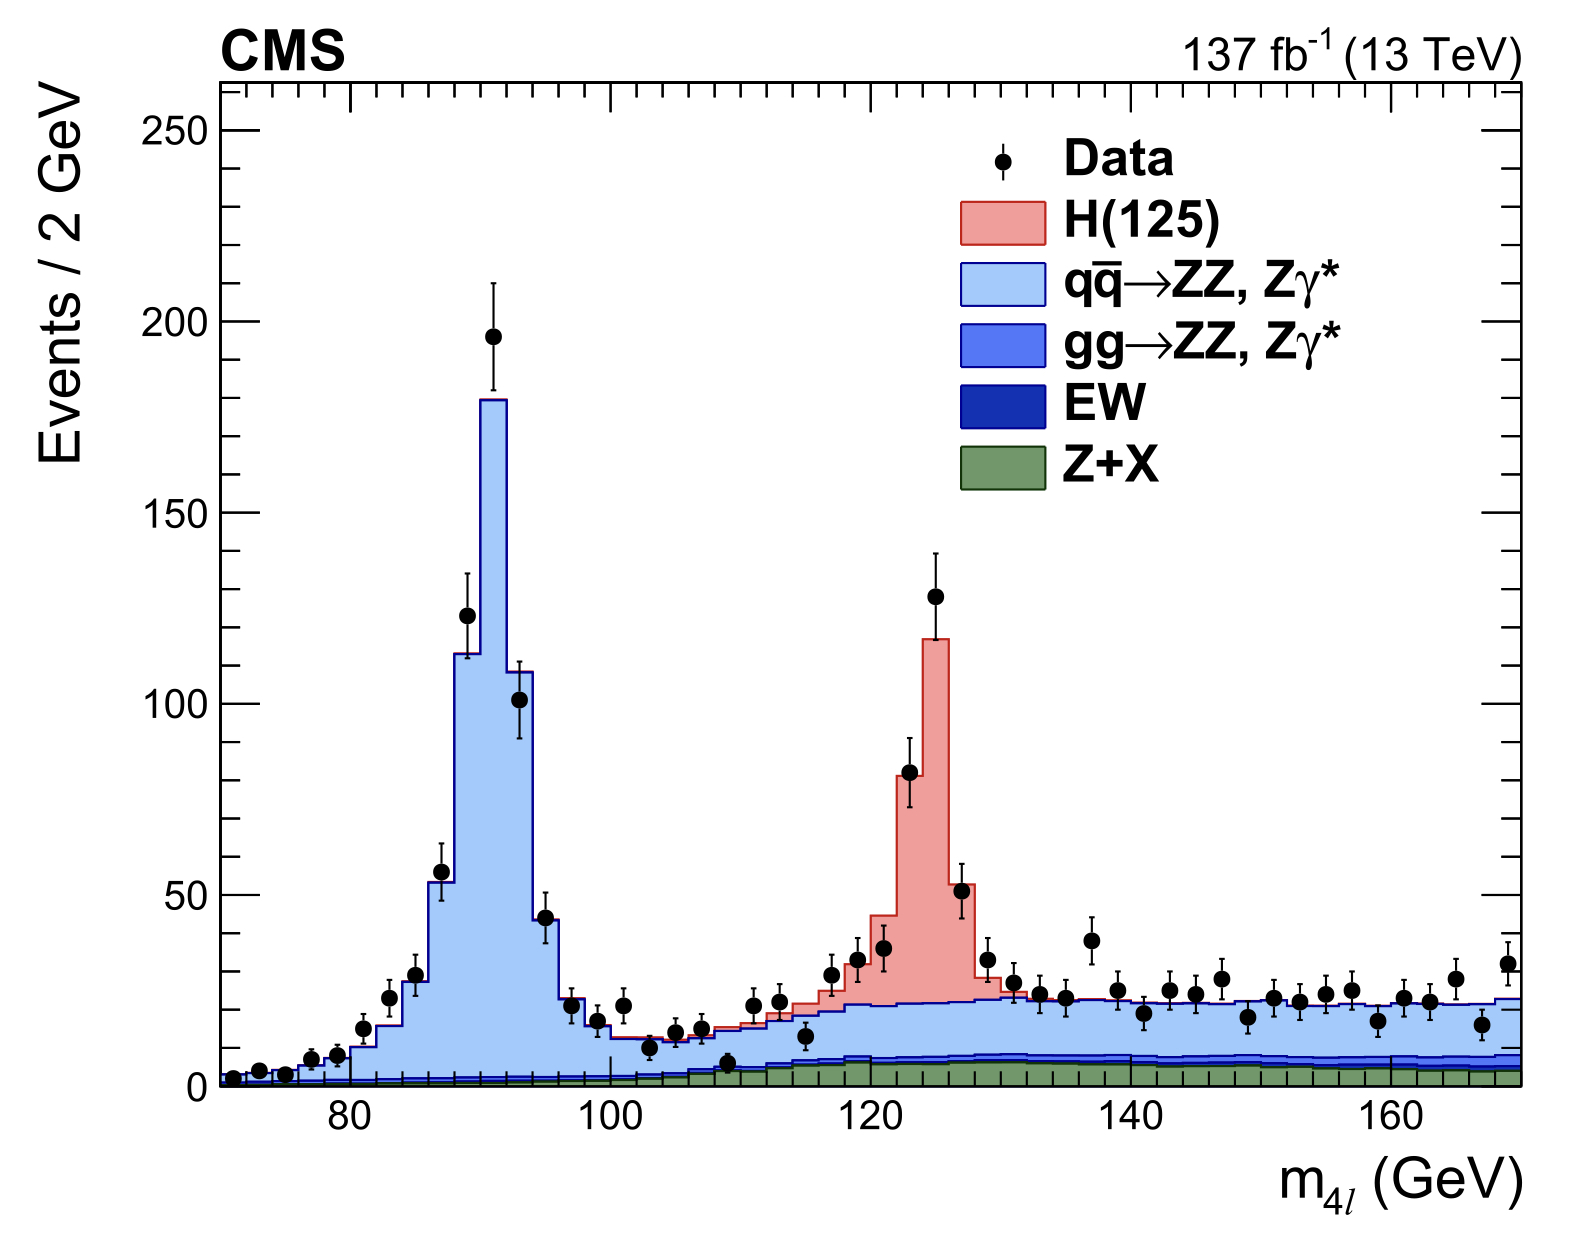
\includegraphics[width=10cm,height=10cm,keepaspectratio]{figures/higgsmassmeas/m4l_FullRun2_epjc.jpeg}
		\caption
			[Distribution of \mfourl from \hzzfourl events using Full Run 2 data.]
			{Distribution of \mfourl from \hzzfourl events using Full Run 2 data.}
        \label{fig:m4l_run2}
\end{figure}

The precision of the measurement of \mH is improved by implementing several techniques:
calculating a per-event matrix element kinematic discriminant,
deriving correction factors for \mfourl uncertainty for various regions of phase space,
reevaluating the lepton \pt values using a \Zone mass constraint,
and constraining the four muon tracks to the selected vertex (\emph{vertex constraint}).
% The implementation of these techniques is discussed in Sec.~\ref{sec:techniques}.
% The first technique is called the \Zone mass constraint, which uses the benefit of the mostly on-shell \Zone mass resonance to reevaluate the momenta of the two leptons that built the \Zone, on a per-event basis.
% This improves the overall lepton momentum resolution, thereby improving the resolution of the \mH peak.
% The second technique is per-event mass uncertainty.
% The third technique is vertex constraint.

% is mostly on-shell as opposed to the \Ztwo.
% Z1 significantly on-shell, but Z2 is mostly off-shell.
% 	- Therefore just perform constraint on mZ1.
% 	- Idea is to reevaluate the lepton
% - Per-event 

Important in any scientific analysis is the careful study of all the associated uncertainties that inherently come with making \emph{any} measurement.
The two main kinds of uncertainties are either \emph{statistical}, which depend on the number of data points used to the make the measurement, or \emph{systematic}, which depend on the instrumentation precision used to make the measurement.
The systematic uncertainties for this analysis include:
\begin{itemize}
	\item \lumiint
	% TODO
	(2.5\%)
	\item Lepton identification and reconstruction efficiencies (
		% TODO
		2.5--9\%)
	\item Lepton energy scale
	% \item BOTH OF THE ABOVE AFFECT SIGNAL AND BKG.
	\item Estimation of the reducible background (40\%).
\end{itemize}
The systematic theoretical uncertainties include:
\begin{itemize}
	\item Renormalization and factorization scale uncertainties.
	\item Choice of the set of parton distribution functions.
	% \item BOTH OF THE ABOVE AFFECT SIGNAL AND BKG
	\item Branching fraction uncertainties for signal and background processes.
\end{itemize}
% These uncertainties are discussed in Sec.~\ref{sec:syst_uncert}.

% TODO: Fix below.
Finally, a likelihood fit is performed on the \mH spectrum to extract the most likely value of \mH.
% The results are summarized in Sec.~\ref{sec:results}.



% The resolution of the peak 
% Ways to improve the 
% Do likelihood fit.

% TODO: Incorporate the below?
% \textbf{FROM THE AN}
% \begin{itemize}
% 	\item TODO:REWORD First, assess what the expected statistical uncertainty will be on \mH using a 1D $\text{pdf} \left( \mfourl \right)$ on the signal events alone (\ie assuming no background).
% 	\item TODO:REWORD Next, add the vertex constraint in reconstruction of muon \pt.
% 	\item TODO:REWORD Then, use the expected \Zone mass line shape for a scalar Higgs boson to refit the momenta of the leptons originating from the \Zone.
% 	\item Next, we include per-event four-lepton mass uncertainties in the mass measurement. 
% 	Events that are assessed to have better four-lepton mass resolution then acquire higher weight in the mass fit.
% 	\item Add the background and assess how it worsens the expected \mH uncertainties.
% 	\item Introduce the kinematic discriminant $\left( \Dkinbkg \right)$, whose purpose is to discriminate signal events from background events.
% 	This discriminant works on a per-event basis using the four-lepton kinematical observables, instead of directly using the four-lepton mass.
% 	In the Higgs boson mass fit, this gives less weight to events with four-lepton kinematic configurations more typical of background than signal.
% 	\item Finally, add all systematic uncertainties to study how they contribute to, \ie propagate into, the total uncertainty on \mH.
% \end{itemize}




% \begin{table}[!htb]	
% 	\centering
% 	% \captionsetup{justification=justified}
% 	\topcaption{Previous Higgs boson mass measurements made by ATLAS and CMS using the \htofourl decay channel.}
% 	\begin{tabular}{|c|c|c|}
% 		\hline			
% 		Collaboration	&	Mass (GeV) \\
% 		\hline
% 		CMS	            &	125.38 $\pm$ 0.14 \\
% 		ATLAS	        &	124.97 $\pm$ 0.24 \\
% 		\hline			
% 	\end{tabular}
% 	\label{tab:cms_vs_atlas}
% \end{table}
% For reference, Table~\ref{tab:cms_vs_atlas} summarizes the previous Higgs boson mass measurements made by ATLAS and CMS collaborations, using the \htofourl decay channel.
